% ============================================================
% CHAPTER 3 -- STUDY AND IMPLEMENTATION OF SPRINT 1 AND SPRINT 2
% ============================================================
\chapter{Marketplace Foundations}
\label{chap:sprints12}
\chaptersommaire
\clearpage

\chapterintro{%
This chapter presents the study and implementation of Sprint~1 and Sprint~2, covering the authentication and access-control foundation, followed by the public marketplace experience.%
}

% ============================================================
% SPRINT 1 — AUTHENTICATION & RBAC
% ============================================================
\section{Sprint 1: Authentication, Profiles and RBAC}

Sprint~1 builds the access foundation. It covers user registration, sign-in, password
recovery, profile management and the role-based access control model on which every
subsequent feature relies.

\subsection{Sprint 1 Backlog}

Table~\ref{tab:sprint1_backlog} summarizes the backlog of the first sprint.

\begin{table}[H]
\centering
\caption{Sprint 1 Backlog}
\renewcommand{\arraystretch}{1.2}
\begin{tabular}{|C{0.6cm}|L{10cm}|C{2.5cm}|}
\hline
\rowcolor{isiBlue}
\textcolor{white}{\textbf{ID}} &
\textcolor{white}{\textbf{User Story}} &
\textcolor{white}{\textbf{Estimation}} \\
\hline
1 & As a visitor, I want to create an account using email/password or OAuth so I can access protected features. & 4 days \\
\hline
2 & As a registered user, I want to sign in and receive a JWT so I can call protected endpoints. & 3 days \\
\hline
3 & As a user, I want to reset my password by email so I can recover my account. & 2 days \\
\hline
4 & As a user, I want to manage my profile so my public page stays up to date. & 2 days \\
\hline
5 & As an administrator, I want each user to belong to a role that grants a specific set of permissions. & 3 days \\
\hline
6 & As an administrator, I want sensitive actions to be logged. & 2 days \\
\hline
\end{tabular}
\label{tab:sprint1_backlog}
\end{table}

\subsection{Sprint 1 Conception}

\subsubsection{Use Case Diagram}

The figure below illustrates the use case diagram relative to Sprint~1.

\begin{figure}[H]
\centering
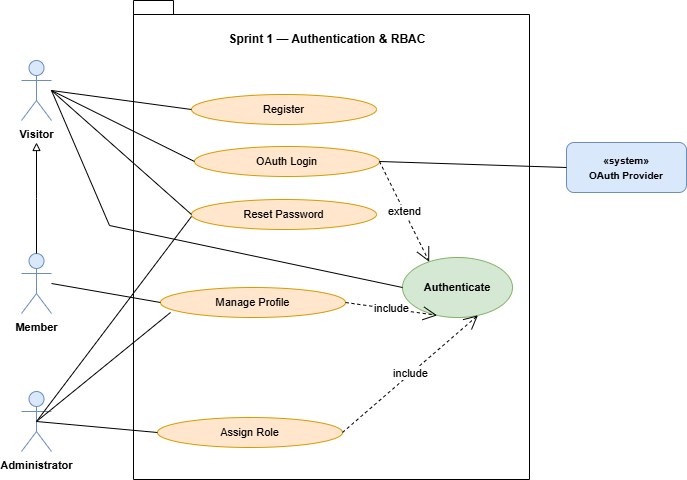
\includegraphics[width=0.9\textwidth]{images/diagrams/uc_s1.png}
\caption{Use case diagram --- Sprint 1}
\label{fig:uc_sprint1}
\end{figure}

\paragraph{Textual description of the use case «Authenticate».}

\begin{table}[H]
\centering
\caption{Use case description: Authenticate}
\label{tab:uc_authenticate}
\renewcommand{\arraystretch}{1.3}
\begin{tabularx}{\textwidth}{|L{3.2cm}|X|}
\hline
\textbf{Use case} & Authenticate \\
\hline
\textbf{Actor} & Registered user \\
\hline
\textbf{Pre-condition} & The user has an active account. \\
\hline
\textbf{Post-condition} & The user holds a valid JWT and can access protected routes. \\
\hline
\textbf{Nominal scenario} &
1. The user opens the sign-in page. \newline
2. The user enters email and password. \newline
3. The system verifies the credentials. \newline
4. The system signs a JWT and returns it to the browser. \newline
5. The browser stores the token and redirects to the marketplace. \\
\hline
\textbf{Alternative scenario} &
3.1. If the credentials are invalid, the system returns an error message. \newline
3.2. Resume at step 2.
\\
\hline
\end{tabularx}
\end{table}

\paragraph{Textual description of the use case «Reset Password».}

\begin{table}[H]
\centering
\caption{Use case description: Reset Password}
\label{tab:uc_reset}
\renewcommand{\arraystretch}{1.3}
\begin{tabularx}{\textwidth}{|L{3.2cm}|X|}
\hline
\textbf{Use case} & Reset Password \\
\hline
\textbf{Actor} & Registered user \\
\hline
\textbf{Pre-condition} & The user has lost access to the account but knows the email. \\
\hline
\textbf{Post-condition} & The password is updated and the user can sign in again. \\
\hline
\textbf{Nominal scenario} &
1. The user requests a reset link by entering an email. \newline
2. The system generates a reset token and emails the reset link. \newline
3. The user opens the link and submits a new password. \newline
4. The system validates the token and stores the new hashed password. \newline
5. A confirmation message is displayed. \\
\hline
\textbf{Alternative scenario} &
4.1. If the token is expired or invalid, an error message is shown. \newline
4.2. The user requests a new reset link.
\\
\hline
\end{tabularx}
\end{table}

\paragraph{Textual description of the use case «Assign Role».}

\begin{table}[H]
\centering
\caption{Use case description: Assign Role}
\label{tab:uc_assign_role}
\renewcommand{\arraystretch}{1.3}
\begin{tabularx}{\textwidth}{|L{3.2cm}|X|}
\hline
\textbf{Use case} & Assign Role \\
\hline
\textbf{Actor} & Administrator \\
\hline
\textbf{Pre-condition} & The administrator is authenticated. \\
\hline
\textbf{Post-condition} & The target user has the chosen role and the associated permissions. \\
\hline
\textbf{Nominal scenario} &
1. The administrator opens the user management page. \newline
2. The administrator selects a user. \newline
3. The administrator chooses a role from the list. \newline
4. The system updates the role assignment and logs the action. \newline
5. A success message is displayed. \\
\hline
\textbf{Alternative scenario} &
3.1. If the administrator does not have the permission to assign the chosen role, an error is shown. \newline
3.2. The administrator picks a different role.
\\
\hline
\end{tabularx}
\end{table}

\subsubsection{Sequence Diagrams}

\paragraph{Sequence diagram «Authenticate».}
When a user attempts to authenticate, the browser sends the credentials to the
\texttt{AuthController}. The system looks up the user record, verifies the password
hash and signs a JWT. The token is returned to the browser, which stores it and
attaches it as a Bearer header on every subsequent call. If credentials are invalid,
the system returns an error and no token is issued.

\begin{figure}[H]
\centering
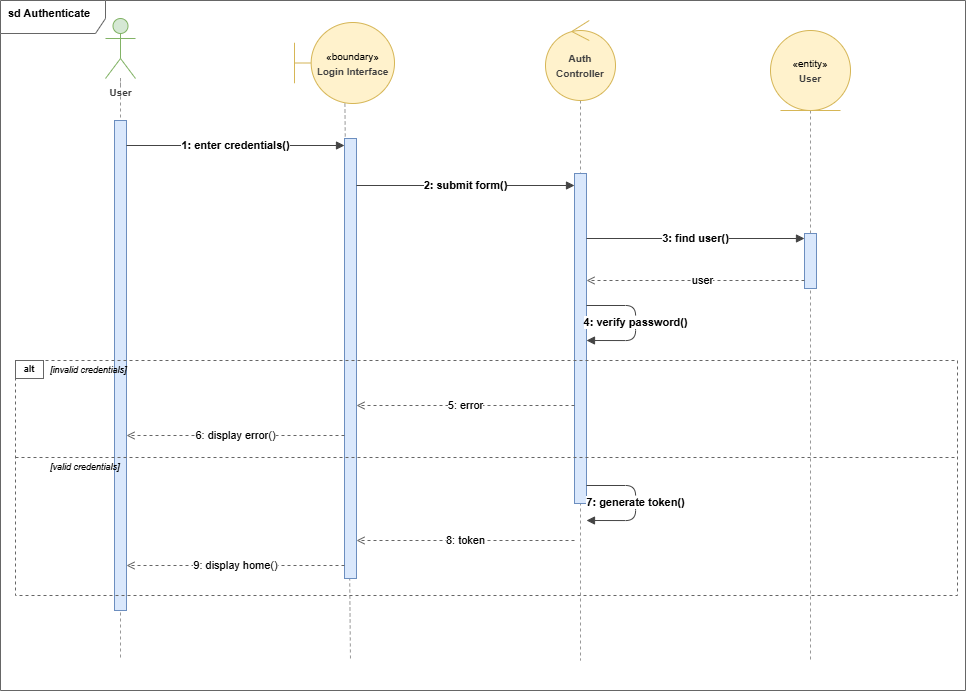
\includegraphics[width=\textwidth]{images/diagrams/seq_auth.png}
\caption{Sequence diagram «Authenticate»}
\label{fig:seq_auth}
\end{figure}

\paragraph{Sequence diagram «Reset Password».}
When a user requests a password reset, the system generates a unique token, stores it
on the user record with an expiry, and sends a reset link by email. When the user
opens the link and submits a new password, the system verifies the token, hashes the
new password and clears the reset token. If the token is missing or expired, the
system rejects the request.

\begin{figure}[H]
\centering
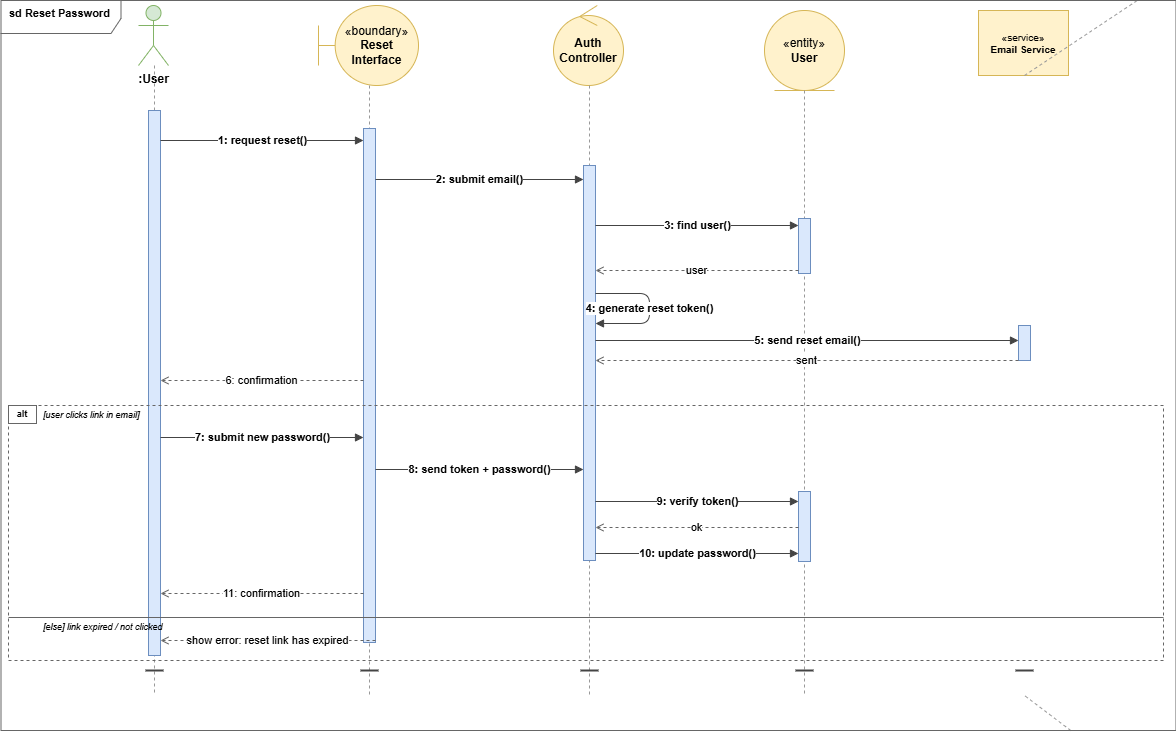
\includegraphics[width=\textwidth]{images/diagrams/seq_reset.png}
\caption{Sequence diagram «Reset Password»}
\label{fig:seq_reset}
\end{figure}

\subsubsection{Class Diagram}

The class diagram of Sprint~1 centres on the \texttt{User} entity linked to the RBAC
trio \texttt{Role}, \texttt{Permission} and \texttt{AuditLog}. A user holds one or
more roles, each role carries a set of permissions, and every sensitive action is
traced in the audit log.

\begin{figure}[H]
\centering
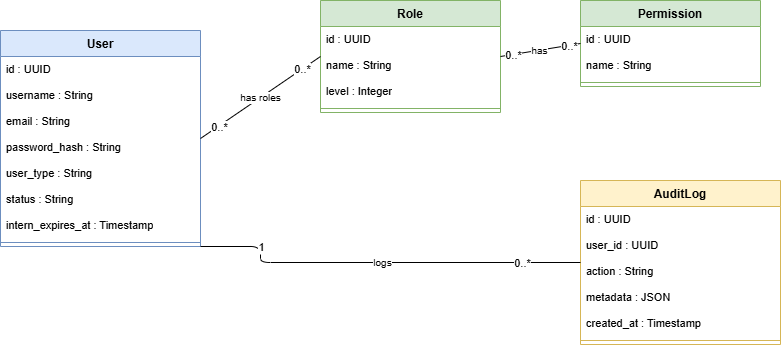
\includegraphics[width=0.95\textwidth]{images/diagrams/class_s1.png}
\caption{Class diagram --- Sprint 1}
\label{fig:class_s1}
\end{figure}

\subsection{Sprint 1 Realization}

In this section we present the interfaces developed during Sprint~1.

\paragraph{«Sign-in interface».}
This interface allows the user to authenticate securely through email and password or
through an OAuth provider. On success, the system stores the JWT and redirects to the
marketplace.

\begin{figure}[H]
\centering
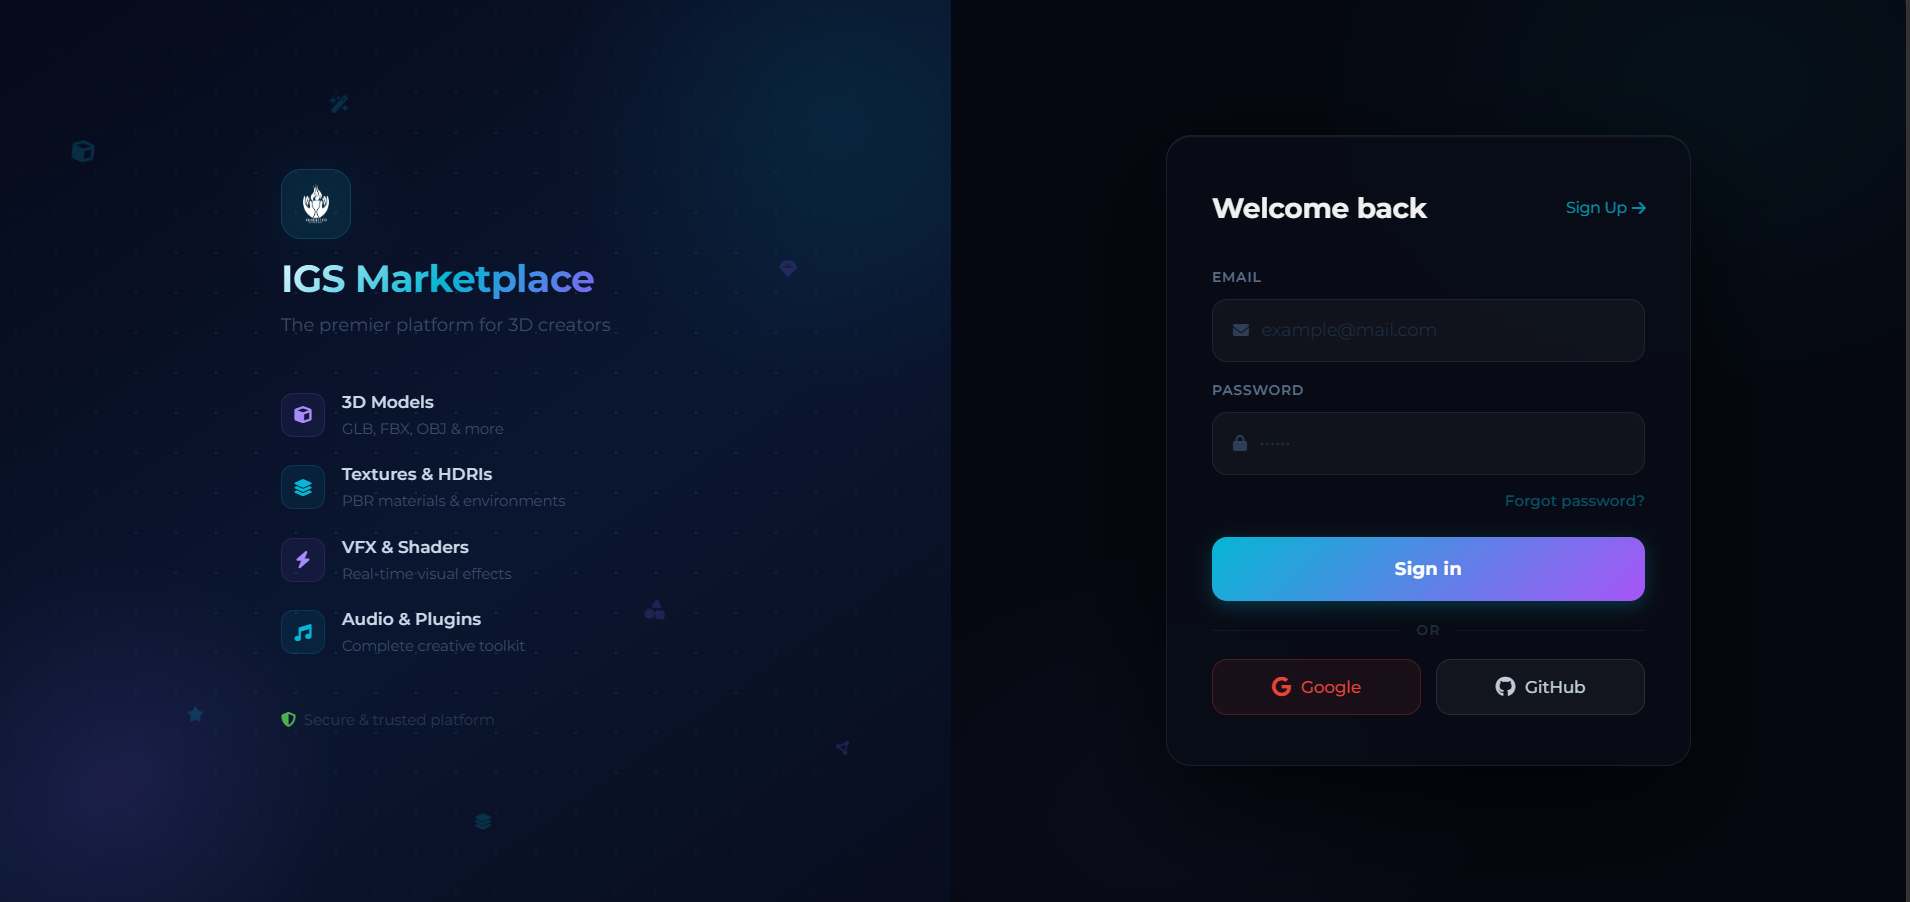
\includegraphics[width=0.8\textwidth]{images/realisation/marketplace/login.png}
\caption{Interface «Sign in»}
\end{figure}

\paragraph{«Sign-up interface».}
This interface lets a new visitor create an account by filling in a short form.
Validation is enforced on the email format and the password strength.

\begin{figure}[H]
\centering
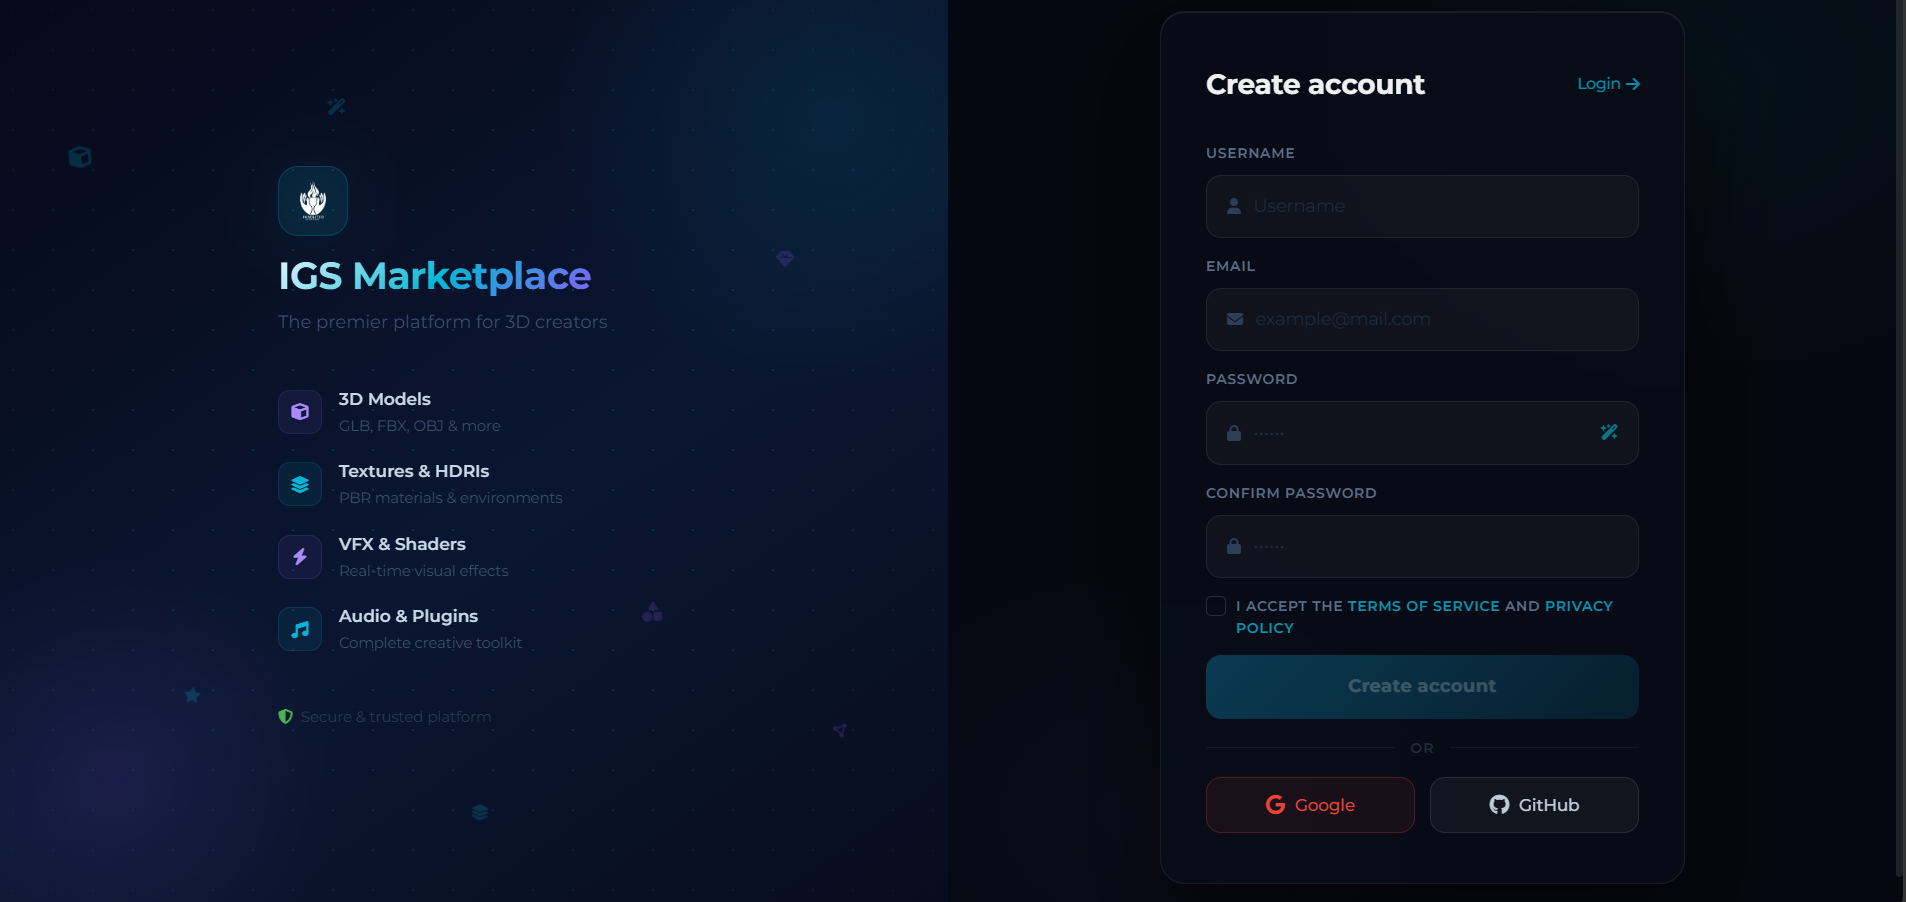
\includegraphics[width=0.8\textwidth]{images/realisation/marketplace/signup.png}
\caption{Interface «Sign up»}
\end{figure}

\paragraph{«Profile management».}
This interface allows the authenticated user to view and update personal information
(avatar, display name, bio, contact details) and to change the account password.

\begin{figure}[H]
\centering
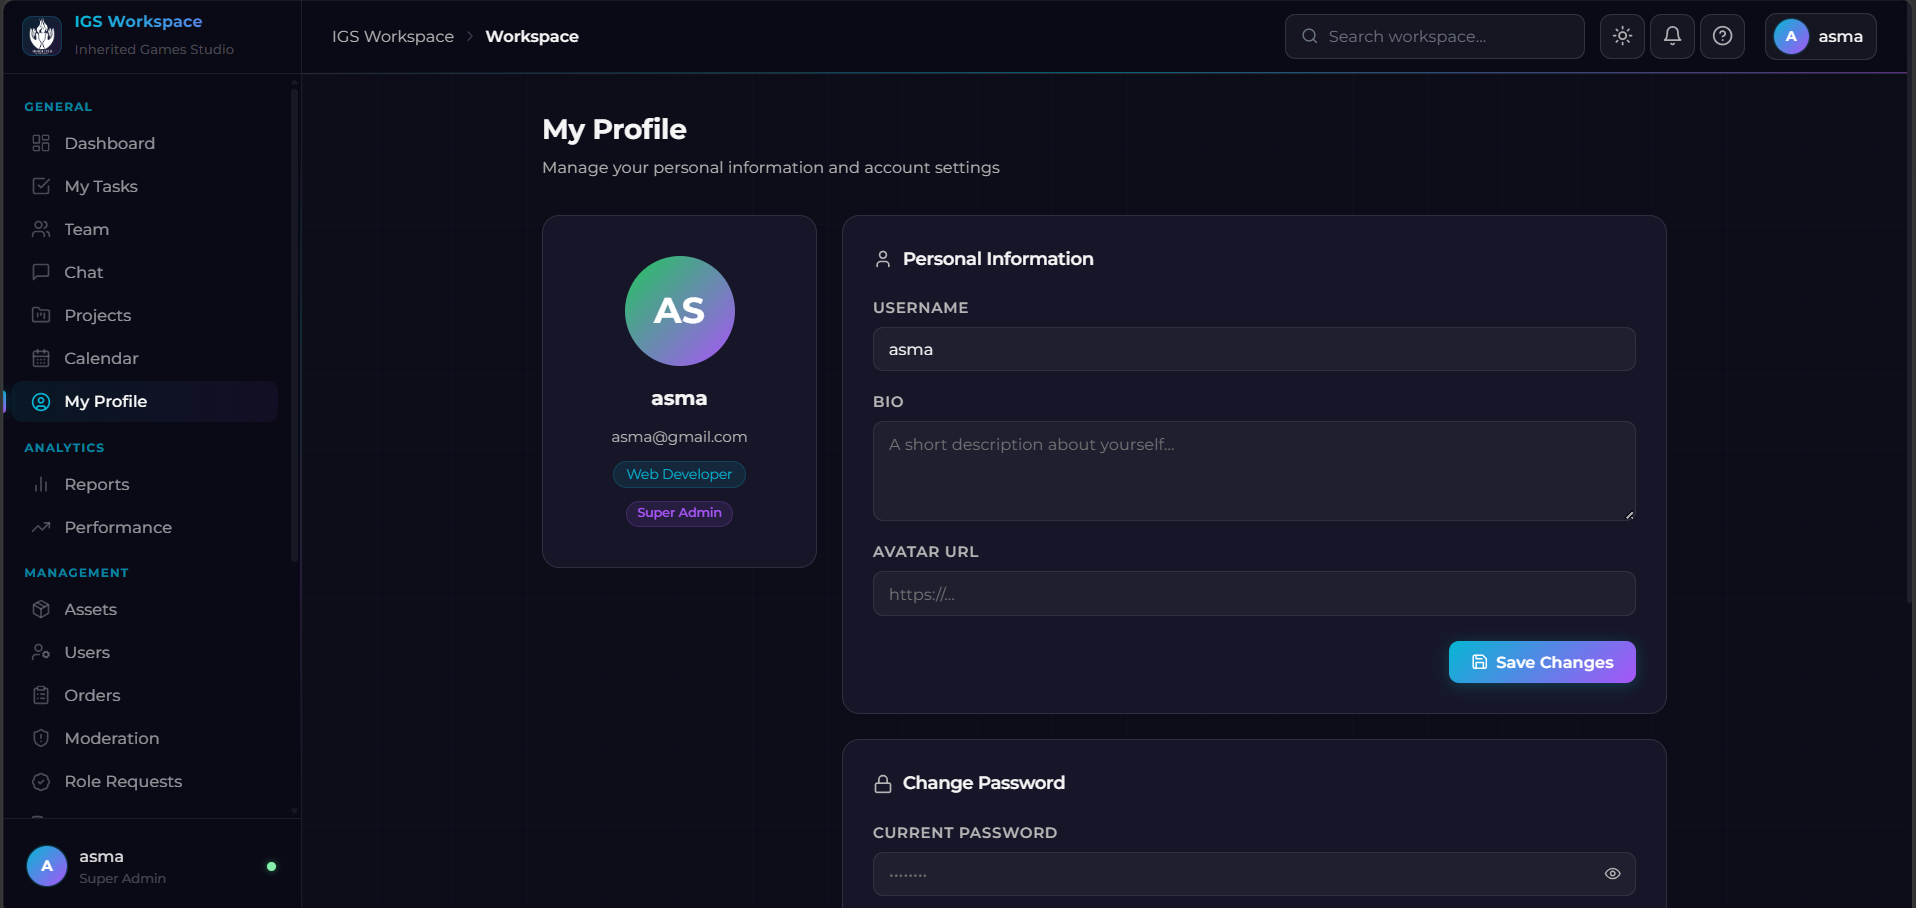
\includegraphics[width=0.8\textwidth]{images/realisation/marketplace/profile.png}
\caption{Interface «Profile»}
\end{figure}

\subsection{Sprint 1 Conclusion}
At the end of Sprint~1 the platform has a working authentication layer with JWT and
OAuth, a profile management page, and a hierarchical RBAC model with six roles. This
foundation conditions every feature delivered in the following sprints.

% ============================================================
% SPRINT 2 — MARKETPLACE CATALOG, PAYMENT, LIBRARY
% ============================================================
\section{Sprint 2: Catalog, Cart, Payment and Library}

Sprint~2 turns the platform into a usable storefront. It delivers the filterable asset
catalog, the interactive 3D and WebXR previews, the shopping cart, the Stripe and
Flouci payment flows and the personal download library.

\subsection{Sprint 2 Backlog}

Table~\ref{tab:sprint2_backlog} summarizes the backlog of the second sprint.

\begin{table}[H]
\centering
\caption{Sprint 2 Backlog}
\renewcommand{\arraystretch}{1.2}
\begin{tabular}{|C{0.6cm}|L{10cm}|C{2.5cm}|}
\hline
\rowcolor{isiBlue}
\textcolor{white}{\textbf{ID}} &
\textcolor{white}{\textbf{User Story}} &
\textcolor{white}{\textbf{Estimation}} \\
\hline
1 & As a visitor, I want to browse a paginated catalogue with filters by category, price and tags. & 3 days \\
\hline
2 & As a visitor, I want to consult an asset detail page with a 3D preview adapted to the asset type. & 4 days \\
\hline
3 & As a member, I want to enter VR / immersive mode for compatible 3D assets so I can inspect them at scale. & 2 days \\
\hline
4 & As a member, I want to add or remove assets from a personal cart. & 2 days \\
\hline
5 & As a member, I want to pay for the cart through Stripe or Flouci and receive instant access. & 4 days \\
\hline
6 & As a member, I want a personal library listing all the assets I can download, with signed-URL downloads. & 3 days \\
\hline
\end{tabular}
\label{tab:sprint2_backlog}
\end{table}

\subsection{Sprint 2 Conception}

\subsubsection{Use Case Diagram}

The figure below illustrates the use case diagram relative to Sprint~2.

\begin{figure}[H]
\centering
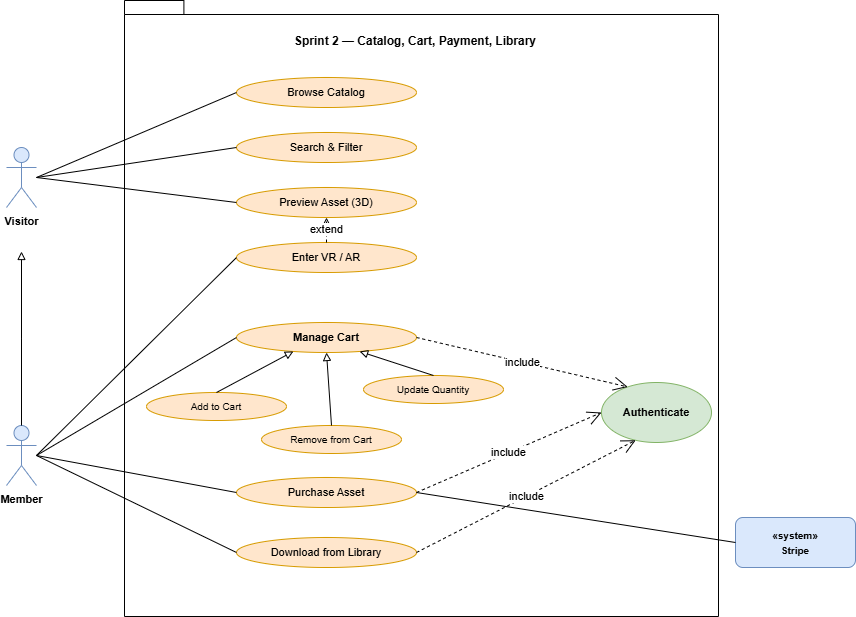
\includegraphics[width=0.9\textwidth]{images/diagrams/uc_s2.png}
\caption{Use case diagram --- Sprint 2}
\label{fig:uc_sprint2}
\end{figure}

\paragraph{Textual description of the use case «Browse and Filter Catalog».}

\begin{table}[H]
\centering
\caption{Use case description: Browse and Filter Catalog}
\label{tab:uc_browse}
\renewcommand{\arraystretch}{1.3}
\begin{tabularx}{\textwidth}{|L{3.2cm}|X|}
\hline
\textbf{Use case} & Browse and Filter Catalog \\
\hline
\textbf{Actor} & Visitor / Member \\
\hline
\textbf{Pre-condition} & The catalog page is accessible. \\
\hline
\textbf{Post-condition} & The catalog displays the filtered list of approved assets. \\
\hline
\textbf{Nominal scenario} &
1. The visitor opens a category page. \newline
2. The visitor applies filters on price, rating or tags. \newline
3. The system queries the catalog with the selected filters. \newline
4. The system returns a paginated list of matching assets. \newline
5. The visitor clicks an asset card to open the detail page. \\
\hline
\textbf{Alternative scenario} &
4.1. If no asset matches the filters, an empty-state message is displayed. \\
\hline
\end{tabularx}
\end{table}

\paragraph{Textual description of the use case «Purchase an Asset».}

\begin{table}[H]
\centering
\caption{Use case description: Purchase an Asset}
\label{tab:uc_purchase}
\renewcommand{\arraystretch}{1.3}
\begin{tabularx}{\textwidth}{|L{3.2cm}|X|}
\hline
\textbf{Use case} & Purchase an Asset \\
\hline
\textbf{Actor} & Member \\
\hline
\textbf{Pre-condition} & The member is authenticated and has at least one asset in the cart. \\
\hline
\textbf{Post-condition} & The order is recorded as paid and the asset is available in the library. \\
\hline
\textbf{Nominal scenario} &
1. The member opens the cart and clicks Checkout. \newline
2. The member selects Stripe or Flouci as payment method. \newline
3. The system creates a payment intent and presents the card form. \newline
4. The payment gateway confirms the transaction. \newline
5. The system records the order, copies the cart items and unlocks the library. \newline
6. A confirmation message is shown. \\
\hline
\textbf{Alternative scenario} &
4.1. If the payment fails, the order stays pending and the library is not unlocked. \newline
4.2. The member can retry from the cart. \\
\hline
\end{tabularx}
\end{table}

\paragraph{Textual description of the use case «Download from Library».}

\begin{table}[H]
\centering
\caption{Use case description: Download from Library}
\label{tab:uc_download}
\renewcommand{\arraystretch}{1.3}
\begin{tabularx}{\textwidth}{|L{3.2cm}|X|}
\hline
\textbf{Use case} & Download from Library \\
\hline
\textbf{Actor} & Member \\
\hline
\textbf{Pre-condition} & The member has at least one asset unlocked in the library. \\
\hline
\textbf{Post-condition} & The asset file is downloaded to the user's machine. \\
\hline
\textbf{Nominal scenario} &
1. The member opens the library page. \newline
2. The member clicks Download on an asset. \newline
3. The system re-checks the access level for the asset. \newline
4. The system generates a signed URL with a one-hour validity. \newline
5. The browser fetches the file directly from cloud storage. \\
\hline
\textbf{Alternative scenario} &
3.1. If the access level is blocked, the system returns a 403 error. \\
\hline
\end{tabularx}
\end{table}

\subsubsection{Sequence Diagrams}

\paragraph{Sequence diagram «Purchase an Asset».}
When a member proceeds to checkout, the backend creates a payment intent at the
gateway and returns the client secret to the browser. The user confirms the card and
the gateway notifies the backend of success. The backend then opens a transaction,
inserts the order, copies the cart items into \texttt{order\_items} with the locked
commission split, grants library access, and returns the confirmation to the browser.

\begin{figure}[H]
\centering
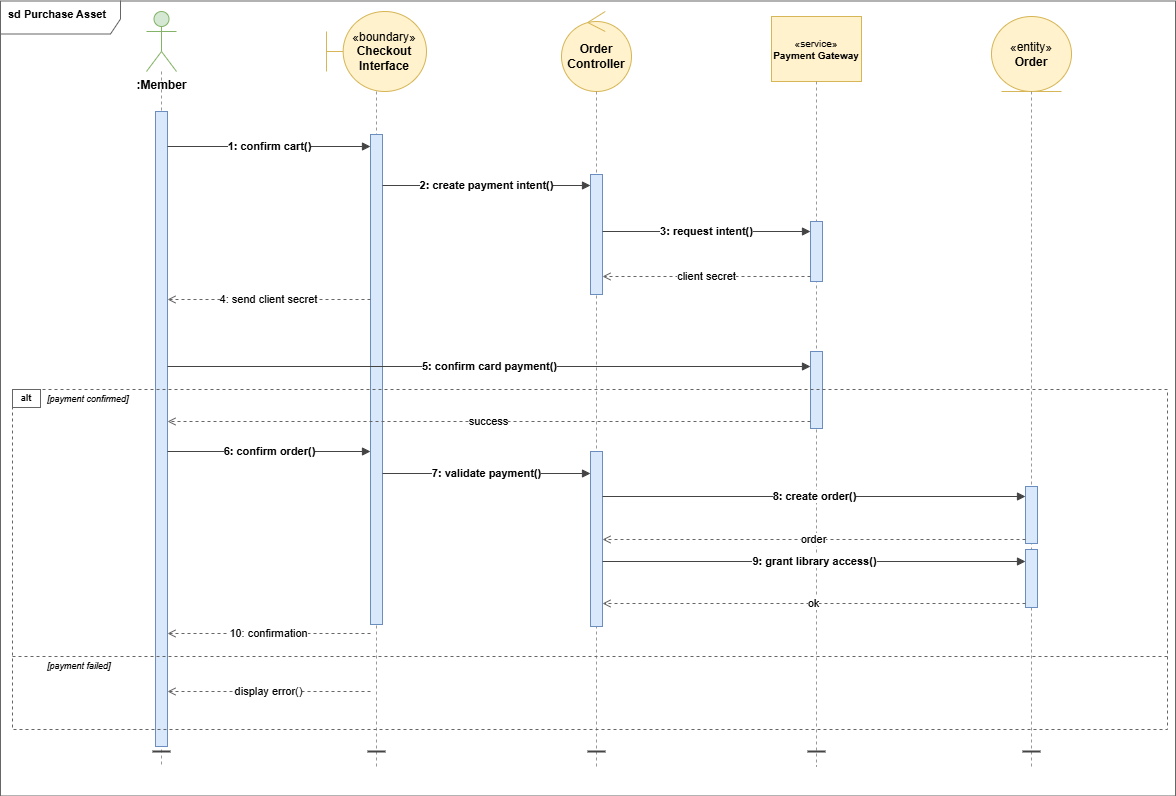
\includegraphics[width=0.95\textwidth]{images/diagrams/seq_payment.png}
\caption{Sequence diagram «Purchase an Asset»}
\label{fig:seq_purchase}
\end{figure}

\paragraph{Sequence diagram «Download from Library».}
When a member clicks Download, the backend re-checks the access level for the asset.
If the access is granted, the backend retrieves the file path and the bucket and
generates a one-hour signed URL through the storage service. The browser uses this
signed URL to fetch the file directly from the CDN, without exposing the bucket path.

\begin{figure}[H]
\centering
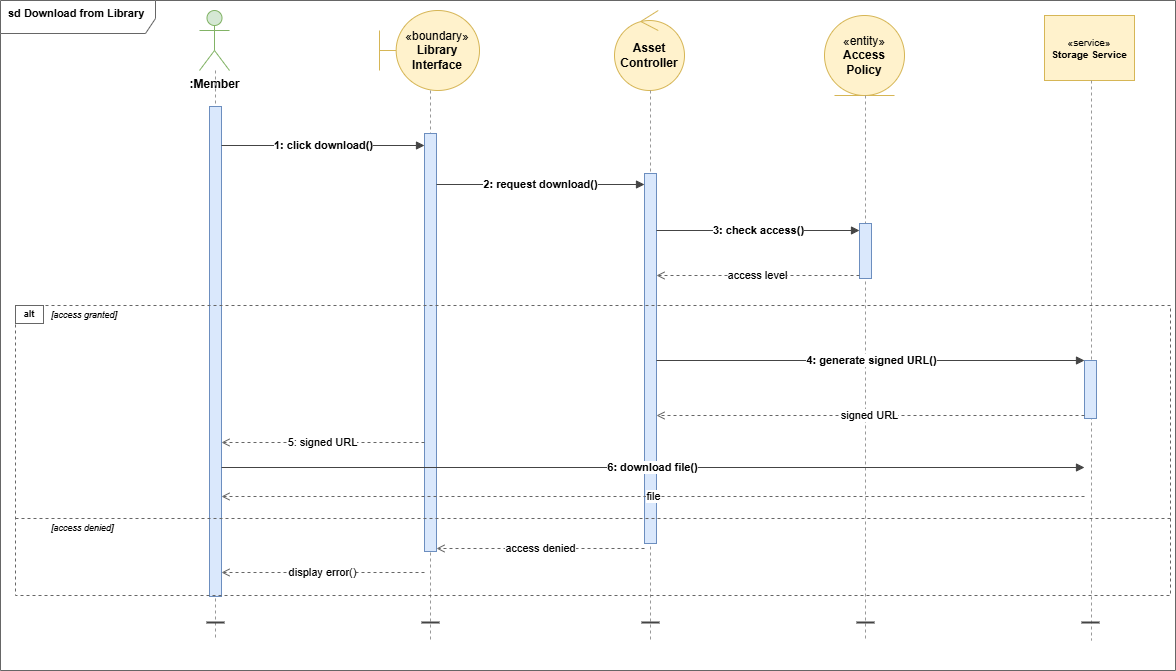
\includegraphics[width=\textwidth]{images/diagrams/seq_download.png}
\caption{Sequence diagram «Download from Library»}
\label{fig:seq_download}
\end{figure}

\subsubsection{Class Diagram}

The class diagram of Sprint~2 introduces the \texttt{Asset} and \texttt{Category}
entities alongside the purchase pipeline: \texttt{CartItem}, \texttt{Order},
\texttt{OrderItem} and \texttt{UserDownload}. Each order item locks the price and
commission split at purchase time so revenue figures remain stable.

\begin{figure}[H]
\centering
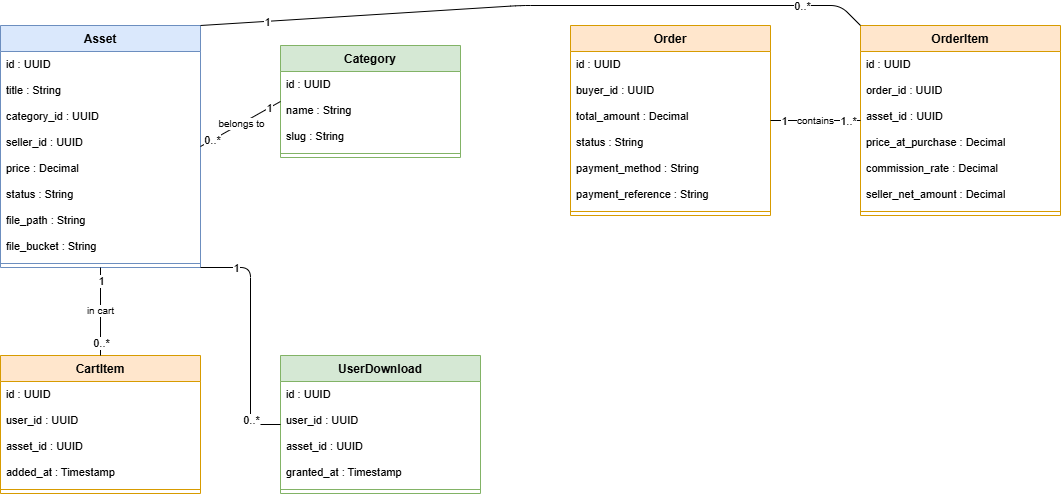
\includegraphics[width=0.95\textwidth]{images/diagrams/class_s2.png}
\caption{Class diagram --- Sprint 2}
\label{fig:class_s2}
\end{figure}

\subsection{Sprint 2 Realization}

In this section we present the interfaces developed during Sprint~2.

\paragraph{«Catalog page».}
This interface lets visitors browse one of the thirteen asset categories. A sidebar
exposes filters by price, rating, tags and file format. Each card shows the
thumbnail, the seller, the price and an interactive preview adapted to the asset
type.

\begin{figure}[H]
\centering
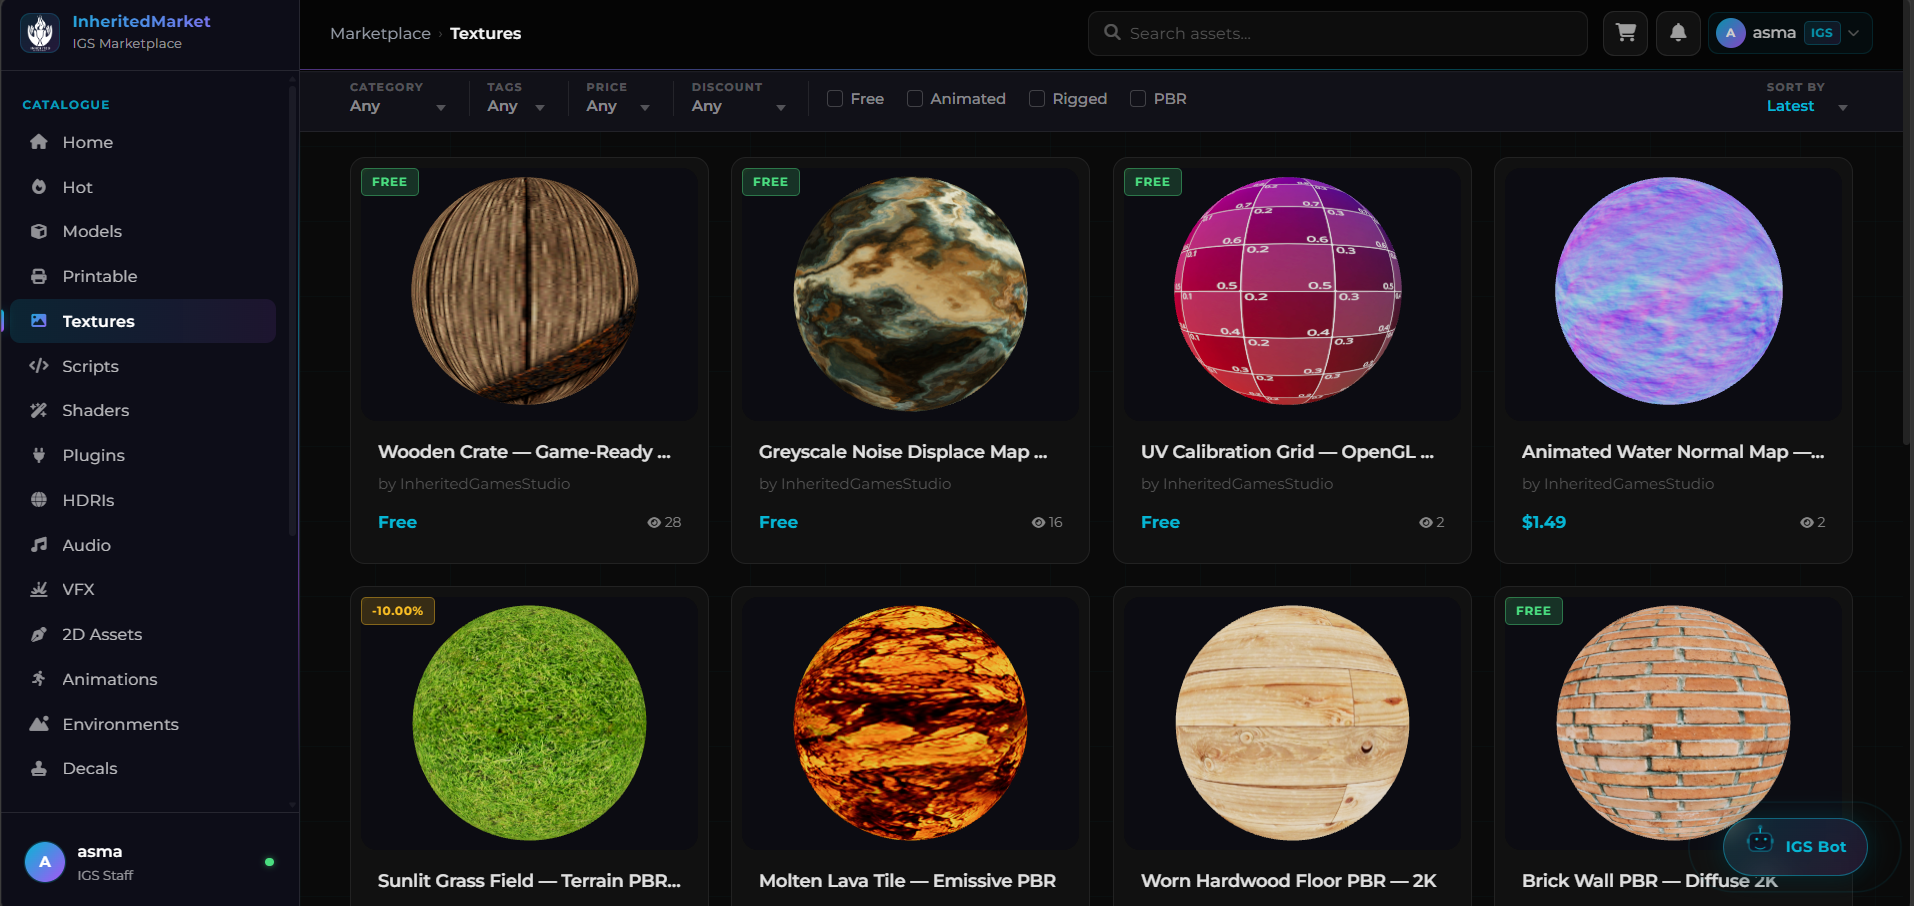
\includegraphics[width=0.85\textwidth]{images/realisation/marketplace/textures page.png}
\caption{Interface «Catalog»}
\end{figure}

\paragraph{«Catalog filters».}
The filter sidebar lets visitors narrow results by price range, rating, tags and file
format. Selections update the catalog grid instantly without a page reload.

\begin{figure}[H]
\centering
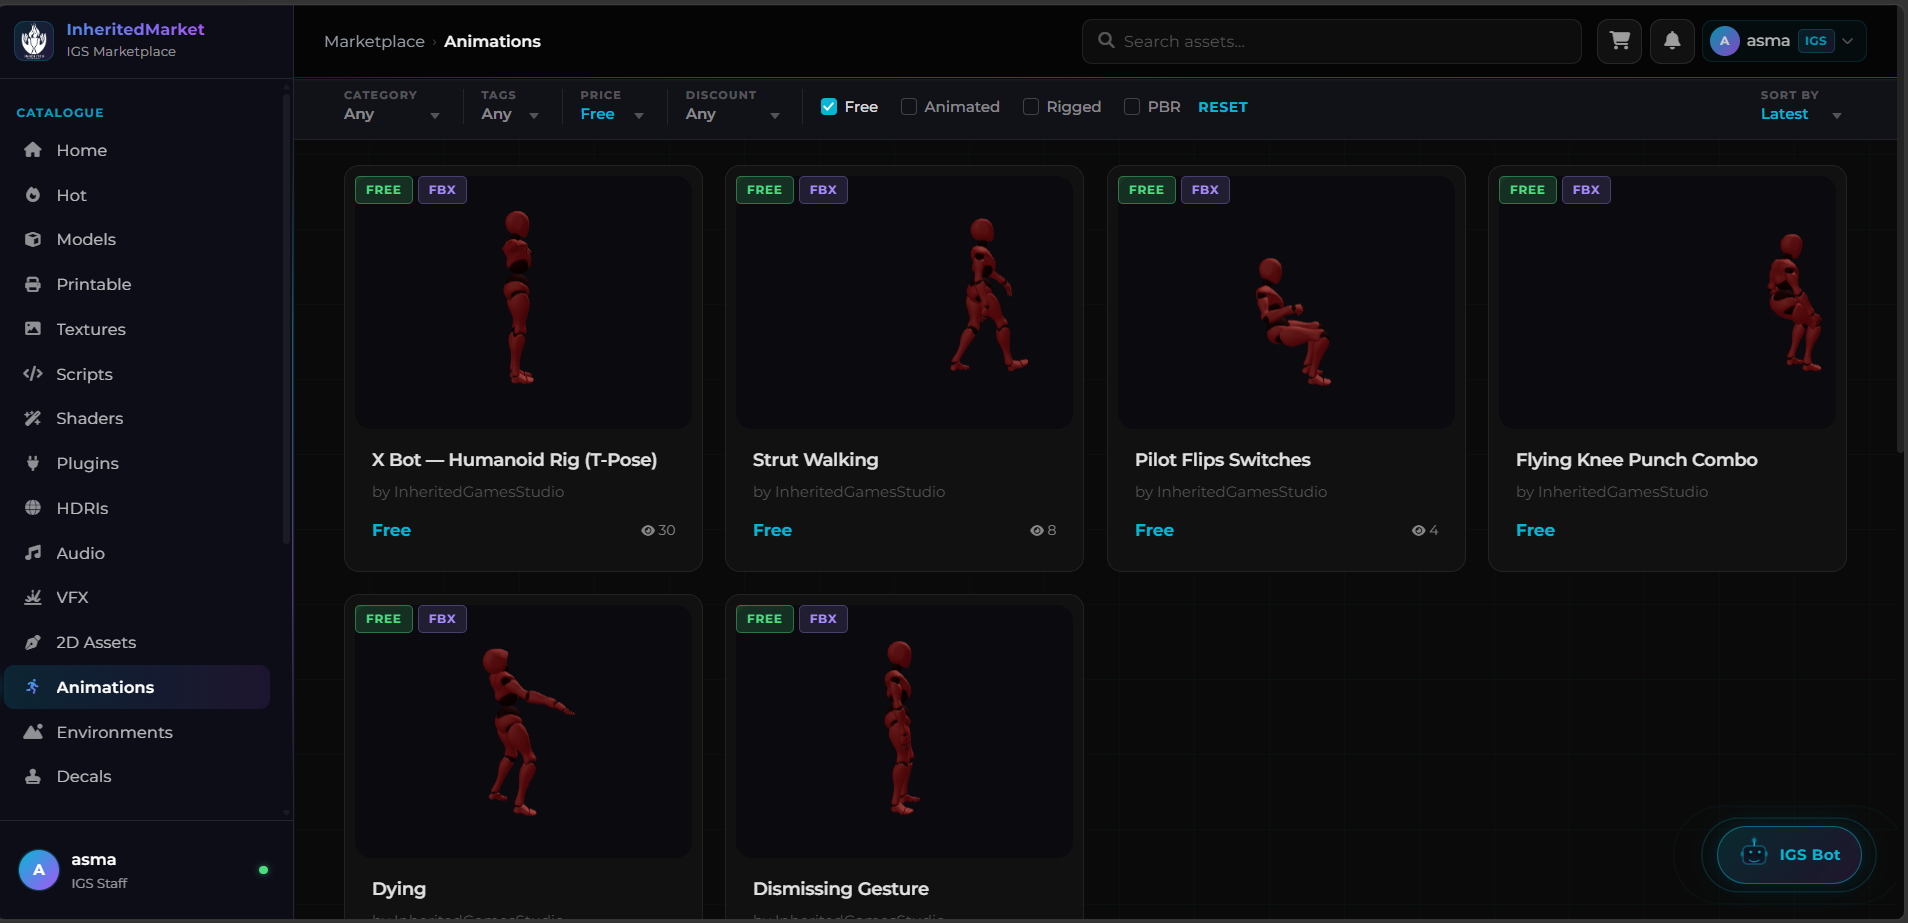
\includegraphics[width=0.85\textwidth]{images/realisation/marketplace/filter.png}
\caption{Interface «Catalog filters»}
\end{figure}

\paragraph{«Shopping cart».}
This interface lists the assets selected by the member. The user can remove an item
or update the quantity, then proceed to checkout with Stripe or Flouci.

\begin{figure}[H]
\centering
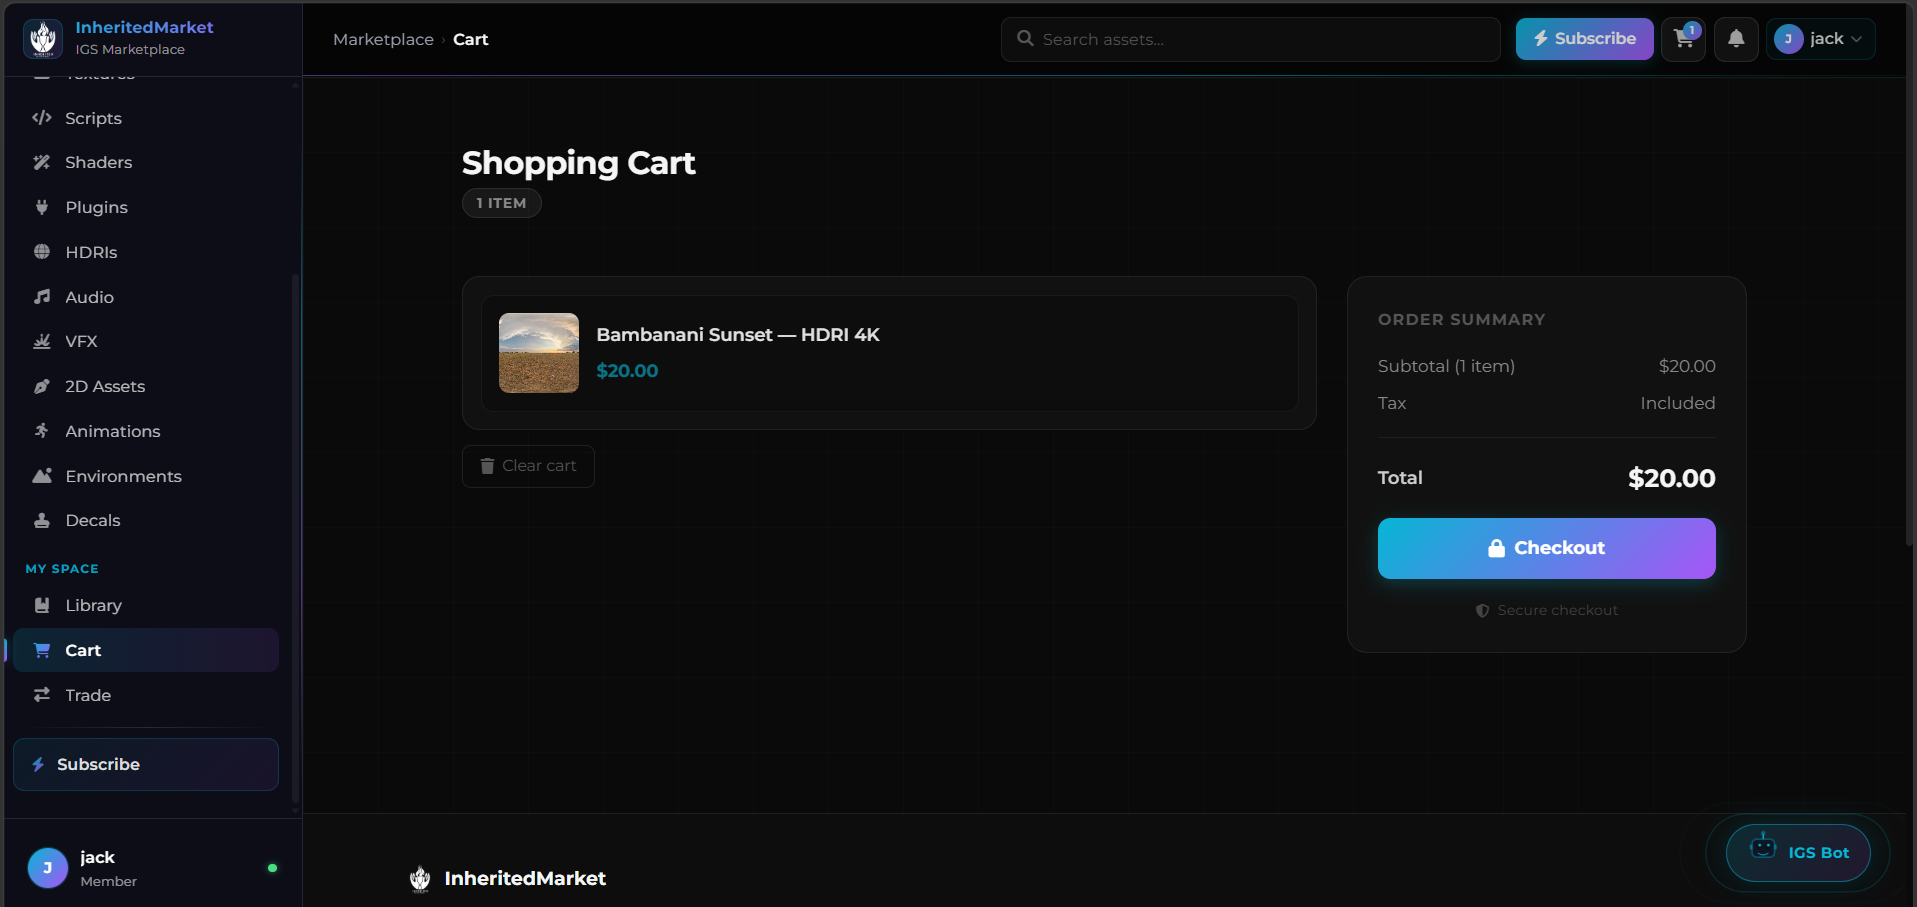
\includegraphics[width=0.85\textwidth]{images/realisation/marketplace/cart.png}
\caption{Interface «Cart»}
\end{figure}

\paragraph{«Library».}
This interface gathers all the assets the member has unlocked (purchased, gifted,
voucher-redeemed or granted by IGS). Each row exposes a Download button that
requests a one-hour signed URL from the backend.

\begin{figure}[H]
\centering
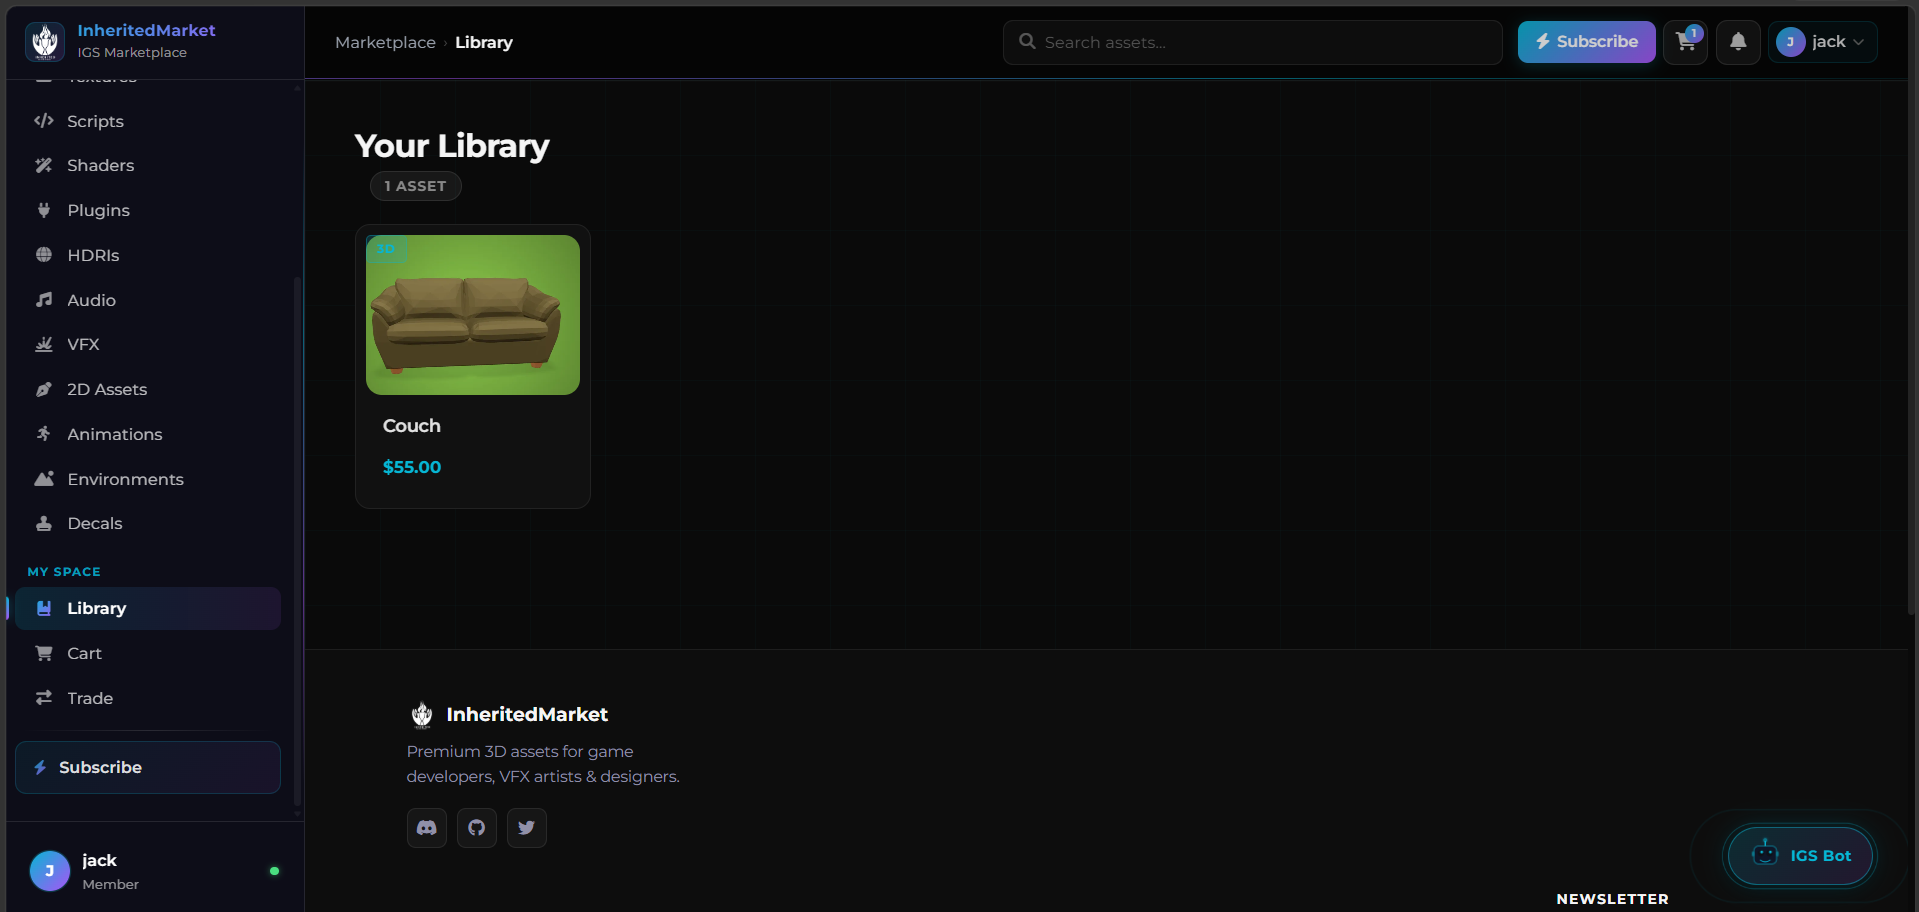
\includegraphics[width=0.85\textwidth]{images/realisation/marketplace/library.png}
\caption{Interface «Library»}
\end{figure}

\subsection{Sprint 2 Conclusion}
At the end of Sprint~2 the public marketplace is fully functional. Visitors can
browse and preview assets in 3D, members can purchase through Stripe or Flouci, and
the personal library exposes time-limited signed downloads.

\section*{Conclusion}
This chapter covered the authentication foundation and the public marketplace implementation across the first two sprints. The following chapter presents Sprint~3 and Sprint~4.
